% -*- coding: utf-8 -*-
% 基于用户提供的 report/main.tex（designed by zcf）调整。
% XeLaTeX 编译；实验正文和表格由 scripts/build_report.py 生成。
\documentclass[UTF8,a4paper,10pt,fontset=fandol]{ctexart}
\usepackage[left=3.17cm,right=3.17cm,top=2.74cm,bottom=2.74cm]{geometry}
\usepackage{amsmath,amssymb}
\usepackage{graphicx,float,booktabs,tabularx,array}
\usepackage{caption,cite,enumitem}
\usepackage{xcolor,listings,fancyhdr,tikz,eso-pic}
\usepackage{xurl}
\usepackage[colorlinks,linkcolor=black,citecolor=black,urlcolor=blue!55!black]{hyperref}
\graphicspath{{../docs/figures/}{./}}
% 优先沿用模板的 Noto 字体；Windows 使用宋体，其他环境回退到 TeX Live 的 Fandol。
\IfFontExistsTF{Noto Serif CJK SC}{
  \setCJKmainfont[AutoFakeBold=2,AutoFakeSlant=0.15]{Noto Serif CJK SC}
}{
  \IfFontExistsTF{SimSun}{
    \setCJKmainfont[BoldFont=SimHei,ItalicFont=KaiTi]{SimSun}
    \setCJKsansfont{SimHei}
    \setCJKfamilyfont{zhkai}[AutoFakeBold=2]{KaiTi}
  }{}
}
\newcommand{\yihao}{\fontsize{26pt}{36pt}\selectfont}
\newcommand{\erhao}{\fontsize{22pt}{28pt}\selectfont}
\newcommand{\xiaoer}{\fontsize{18pt}{24pt}\selectfont}
\newcommand{\sanhao}{\fontsize{16pt}{24pt}\selectfont}
\newcommand{\sihao}{\fontsize{14pt}{21pt}\selectfont}
\newcommand{\xiaosi}{\fontsize{12pt}{18pt}\selectfont}
\newcommand{\wuhao}{\fontsize{10.5pt}{15.75pt}\selectfont}
\ctexset{
  section={name={,、},number=\chinese{section},format=\large\bfseries\raggedright},
  subsection={name={（,）},number=\chinese{subsection},format=\normalsize\bfseries\raggedright},
  subsubsection={name={,.},number=\arabic{subsubsection}}
}
\setlength{\headheight}{16pt}
\pagestyle{fancy}
\fancyhf{}
\fancyhead[L]{\small\kaishu\nouppercase{\leftmark}}
\fancyhead[R]{\small\kaishu 文本分类实验报告}
\fancyfoot[C]{\thepage}
\renewcommand{\headrulewidth}{0.1pt}
\renewcommand{\footrulewidth}{0pt}
\newcommand{\HRule}{\rule{\linewidth}{0.5mm}}
\captionsetup{font=small,labelfont=bf}
\setlength{\parskip}{0.3em}
\setlength{\emergencystretch}{2em}
\raggedbottom
\lstset{basicstyle=\small\ttfamily,breaklines=true,frame=single,numbers=left,numberstyle=\tiny}
\newcommand{\watermark}{%
  \AddToShipoutPictureBG{%
    \begin{tikzpicture}[remember picture,overlay]
      \node[rotate=60,scale=10,text=black!4] at (current page.center) {NKU};
    \end{tikzpicture}}}
\hypersetup{pdftitle={NYT 新闻文本分类实验报告},pdfsubject={作业一 词袋表示 词向量与 BERT 微调}}
\begin{document}
\begin{titlepage}
  \begin{center}
    
\includegraphics[width=0.8\textwidth]{NKU.png}\\[0.8cm]
    {\Huge\kaishu\bfseries 南\quad 开\quad 大\quad 学}\\[0.7cm]
    {\huge\kaishu\bfseries 计\quad 算\quad 机\quad 学\quad 院}\\[0.7cm]
    {\Large\bfseries 作业一实验报告}\\[0.7cm]
    \HRule\\[0.7cm]
    {\LARGE\bfseries NYT 新闻文本分类}\\[0.35cm]
    {\large 词袋表示、词向量与 BERT 微调}\\[0.5cm]
    \HRule\\[1.3cm]
    {\large 数据集：NYT 与 AG News}\\[0.4cm]
    {\large 实验内容：七组文本分类方法对比}\\[0.4cm]
    {\large 评价指标：Accuracy 与 Macro-F1}
    \vfill
    {\Large\today}
  \end{center}
\end{titlepage}
\pagenumbering{Roman}
\thispagestyle{plain}
\renewcommand{\abstractname}{\kaishu\sihao\textbf{摘要}}
\begin{abstract}
  本实验使用同一 NYT 测试集比较七种方法。此次单次实验中，TF-IDF 的测试 Macro-F1 最高，为 0.9812，Accuracy 为 0.9922。全部结果来自实际训练；每条测试预测、划分行号和运行参数均随仓库保存。

  \par\medskip\noindent\textbf{关键词：}文本分类；词袋模型；Word2Vec；GloVe；BERT
\end{abstract}
\tableofcontents
\clearpage
\pagenumbering{arabic}
\watermark
\wuhao
\section{数据与实验范围}

NYT 共 11,519 篇新闻，包含 business、politics、sports 三类；AG News 共 90,000 篇，仅用于训练其中一组 Word2Vec。固定随机种子 42，以分层随机方式打乱并按约 80\% / 10\% / 10\% 划分。

\begin{table}[H]
\centering\small
\setlength{\tabcolsep}{4pt}
\renewcommand{\arraystretch}{1.2}
\caption{NYT 统一数据划分}
\label{tab:result1}
\begin{tabularx}{\linewidth}{>{\hsize=0.82474\hsize\linewidth=\hsize\raggedright\arraybackslash}X>{\hsize=1.03093\hsize\linewidth=\hsize\raggedright\arraybackslash}X>{\hsize=1.03093\hsize\linewidth=\hsize\raggedright\arraybackslash}X>{\hsize=1.03093\hsize\linewidth=\hsize\raggedright\arraybackslash}X>{\hsize=1.08247\hsize\linewidth=\hsize\raggedright\arraybackslash}X}
\toprule
集合 & business & politics & sports & 总数 \\
\midrule
训练 & 1143 & 1161 & 6911 & 9215 \\
验证 & 143 & 145 & 864 & 1152 \\
测试 & 143 & 145 & 864 & 1152 \\
\bottomrule
\end{tabularx}
\end{table}

类别明显不平衡。仅预测 sports 的基线 Accuracy 为 0.7500，Macro-F1 为 0.2857。因此主要依据 Macro-F1 比较对少数类别的识别能力，同时报告 Accuracy。

要求说明：Task 1 总述写“三种”，但正文只列出 Binary 和 Word Frequency。本实验完成这两项，并补充 TF-IDF 作为第三种；此项属于对原文歧义的明确实现选择。

原 NYT 中有 72 条重复文本记录。保持原始样本开展规定的随机划分，并单独审计跨集合重复，避免隐瞒可能造成的乐观偏差。


\section{表示方法与训练设置}

词袋与词向量实验使用同一分词规则：转为小写，提取英文词并保留词内撇号，不移除停用词。BERT 则使用其预训练 WordPiece tokenizer。Accuracy 是正确预测比例；Macro-F1 是三个类别各自 F1 的算术平均，零分母按 0 处理。


\begin{equation}
\mathrm{Accuracy}=\frac{1}{N}\sum_{i=1}^{N}\mathbf{1}[\hat y_i=y_i],
\qquad
\mathrm{MacroF1}=\frac{1}{K}\sum_{k=1}^{K}F1_k.
\end{equation}

\begin{table}[H]
\centering\small
\setlength{\tabcolsep}{4pt}
\renewcommand{\arraystretch}{1.2}
\caption{文本表示方法}
\label{tab:result2}
\begin{tabularx}{\linewidth}{>{\hsize=0.45361\hsize\linewidth=\hsize\raggedright\arraybackslash}X>{\hsize=1.54639\hsize\linewidth=\hsize\raggedright\arraybackslash}X}
\toprule
方法 & 文档表示与参数 \\
\midrule
Binary BoW & 词出现则为 1，否则为 0。完整训练集词表。 \\
Word Frequency & 记录每个词在文档中的出现次数，不进行长度归一化。 \\
TF-IDF & tf × [log((1+N)/(1+df))+1]，随后做文档 L2 归一化。 \\
GloVe & Stanford glove.6B.100d，400,000 个词，100 维预训练词向量。 \\
Word2Vec AG & 全部 AG 文本；Skip-gram，100 维，窗口 5，负采样 5。 \\
Word2Vec NYT & 仅 NYT 训练集文本；与 AG 模型使用相同参数。 \\
\bottomrule
\end{tabularx}
\end{table}


设 $c_{d,i}$ 为词 $i$ 在文档 $d$ 中的次数，三种词袋表示分别为
\begin{align}
x^{\mathrm{binary}}_{d,i}&=\mathbf{1}[c_{d,i}>0],\\
x^{\mathrm{count}}_{d,i}&=c_{d,i},\\
x^{\mathrm{tfidf}}_{d,i}&=c_{d,i}\left[\log\frac{1+N_{\mathrm{train}}}{1+df_i}+1\right].
\end{align}
其中 $df_i$ 仅在训练集统计；TF-IDF 向量随后进行 $L_2$ 归一化。

两组 Word2Vec 最低词频为 5，训练 10 轮；使用单 worker、固定种子和稳定词哈希。词向量方法对文档内所有有效词向量取算术平均，重复出现的词重复计入；跳过 OOV，全 OOV 文档使用零向量。100 维特征标准化仅在训练集上拟合。\cite{mikolov2013efficient,pennington2014glove}


设有效词集合（保留重复出现）为 $D_{\mathrm{valid}}$，则文档表示为
\begin{equation}
\mathbf e(d)=\frac{1}{|D_{\mathrm{valid}}|}
\sum_{w\in D_{\mathrm{valid}}}\mathbf e(w).
\end{equation}
当 $|D_{\mathrm{valid}}|=0$ 时使用零向量。

六组传统方法统一使用 Logistic Regression（L2 正则，lbfgs，最多 3000 次迭代）。在 C=\{0.1,1,10\} 中只依据验证 Macro-F1 选择，平局取较小 C；所选模型仅训练于训练集，不再合并验证集。词表、IDF、标准化和 NYT Word2Vec 都不拟合验证或测试文本。

\begin{table}[H]
\centering\small
\setlength{\tabcolsep}{4pt}
\renewcommand{\arraystretch}{1.2}
\caption{传统模型的验证集选择}
\label{tab:result3}
\begin{tabularx}{\linewidth}{>{\hsize=1.07216\hsize\linewidth=\hsize\raggedright\arraybackslash}X>{\hsize=1.03093\hsize\linewidth=\hsize\raggedright\arraybackslash}X>{\hsize=0.70103\hsize\linewidth=\hsize\raggedright\arraybackslash}X>{\hsize=1.19588\hsize\linewidth=\hsize\raggedright\arraybackslash}X}
\toprule
方法 & 词表或向量维数 & 所选 C & 验证 Macro-F1 \\
\midrule
Binary BoW & 64285 & 1.0 & 0.9635 \\
Frequency & 64285 & 0.1 & 0.9591 \\
TF-IDF & 64285 & 10.0 & 0.9639 \\
GloVe & 100 & 0.1 & 0.9523 \\
Word2Vec AG & 100 & 0.1 & 0.9465 \\
Word2Vec NYT & 100 & 1.0 & 0.9632 \\
\bottomrule
\end{tabularx}
\end{table}

BERT 使用 google-bert/bert-base-uncased，全参数微调。max\_length=64（含特殊 token），完整训练 3 轮；批量 16、累积 2、AdamW 学习率 2e-5、权重衰减 0.01、10\% warmup 后线性衰减、梯度裁剪 1.0。bias 与 LayerNorm 权重不做衰减。CUDA 上使用 FP16。\cite{devlin2019bert,bertmodel}


\section{统一测试集结果}

\begin{table}[H]
\centering\small
\setlength{\tabcolsep}{4pt}
\renewcommand{\arraystretch}{1.2}
\caption{NYT 测试集性能}
\label{tab:result4}
\begin{tabularx}{\linewidth}{>{\hsize=1.19588\hsize\linewidth=\hsize\raggedright\arraybackslash}X>{\hsize=0.90722\hsize\linewidth=\hsize\raggedright\arraybackslash}X>{\hsize=0.90722\hsize\linewidth=\hsize\raggedright\arraybackslash}X>{\hsize=0.98969\hsize\linewidth=\hsize\raggedright\arraybackslash}X}
\toprule
方法 & Accuracy & Macro-F1 & 运行秒数 \\
\midrule
Binary BoW & 0.9905 & 0.9754 & 6.9 \\
Frequency & 0.9887 & 0.9738 & 17.1 \\
TF-IDF & 0.9922 & 0.9812 & 7.5 \\
GloVe & 0.9878 & 0.9715 & 11.7 \\
Word2Vec AG & 0.9835 & 0.9581 & 147.3 \\
Word2Vec NYT & 0.9896 & 0.9731 & 224.3 \\
BERT & 0.9809 & 0.9589 & 218.8 \\
\bottomrule
\end{tabularx}
\end{table}

\begin{figure}[H]
\centering
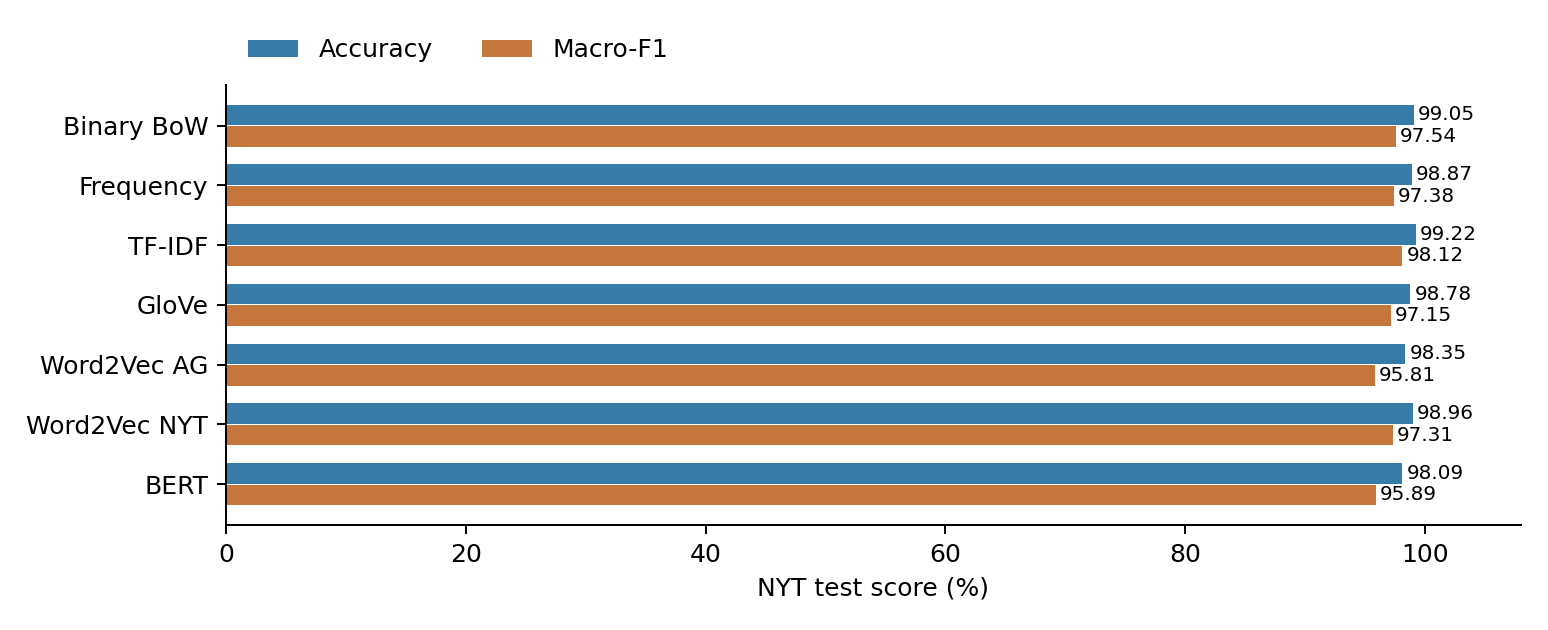
\includegraphics[width=0.98\linewidth]{comparison.png}
\caption{七种方法的统一测试集性能}
\end{figure}

运行时间包括各方法特征构建、训练、验证和预测等步骤，不含预训练资源下载。部分任务并行运行，且硬件与模型结构不同，因此时间仅描述本次运行，不作为严格速度基准。

传统方法中 TF-IDF 的测试 Macro-F1 最高。BERT 与它的差值为 -0.0223。这是固定种子下的描述性比较，未进行多种子重复或显著性检验，不能据此断言某方法在所有数据上更好。

词袋模型保留直接区分类别的关键词；TF-IDF 降低常见词权重。平均词向量压缩到 100 维，能利用词之间的语义联系，但丢失词序，也可能稀释少数关键句。BERT 建模上下文，不过本作业只允许 64 个 token，长新闻的后续信息会被截断。


\section{词向量覆盖与 BERT 训练}

\begin{table}[H]
\centering\small
\setlength{\tabcolsep}{4pt}
\renewcommand{\arraystretch}{1.2}
\caption{词向量 token 覆盖率}
\label{tab:result5}
\begin{tabularx}{\linewidth}{>{\hsize=0.90722\hsize\linewidth=\hsize\raggedright\arraybackslash}X>{\hsize=1.11340\hsize\linewidth=\hsize\raggedright\arraybackslash}X>{\hsize=1.11340\hsize\linewidth=\hsize\raggedright\arraybackslash}X>{\hsize=0.86598\hsize\linewidth=\hsize\raggedright\arraybackslash}X}
\toprule
词向量 & 训练 token 覆盖率 & 测试 token 覆盖率 & 测试全 OOV 文档 \\
\midrule
GloVe & 98.13\% & 98.12\% & 0 \\
Word2Vec AG & 95.78\% & 95.78\% & 0 \\
Word2Vec NYT & 98.91\% & 98.51\% & 0 \\
\bottomrule
\end{tabularx}
\end{table}

AG Word2Vec 与 NYT Word2Vec 的测试 Macro-F1 分别为 0.9581 和 0.9731。领域、语料长度与规模、词覆盖和低频词过滤同时变化，因此性能差异不能单独归因于“同领域”这一因素。覆盖率按词出现次数计算，而非不同词类型数量。

\begin{table}[H]
\centering\small
\setlength{\tabcolsep}{4pt}
\renewcommand{\arraystretch}{1.2}
\caption{BERT 三轮训练记录}
\label{tab:result6}
\begin{tabularx}{\linewidth}{>{\hsize=0.55670\hsize\linewidth=\hsize\raggedright\arraybackslash}X>{\hsize=1.17526\hsize\linewidth=\hsize\raggedright\arraybackslash}X>{\hsize=1.26804\hsize\linewidth=\hsize\raggedright\arraybackslash}X}
\toprule
Epoch & 训练平均损失 & 验证 Macro-F1 \\
\midrule
1 & 0.2847 & 0.9173 \\
2 & 0.0506 & 0.9433 \\
3 & 0.0179 & 0.9480 \\
\bottomrule
\end{tabularx}
\end{table}

\begin{figure}[H]
\centering
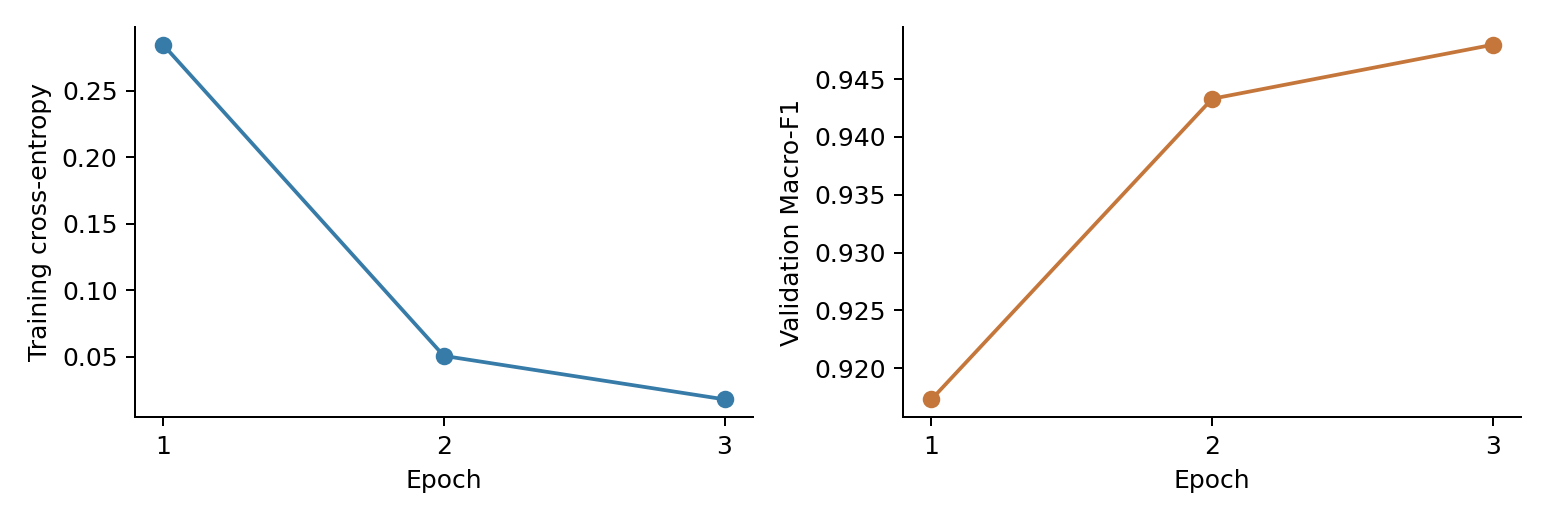
\includegraphics[width=0.98\linewidth]{bert_history.png}
\caption{BERT 三轮训练损失与验证 Macro-F1}
\end{figure}

BERT 完成三轮训练后，依据验证 Macro-F1 选取第 3 轮 checkpoint。测试集不参与轮次选择。完整曲线数据保存在 results/bert\_history.json。

由于模型只观察新闻开头，标题和导语可能携带较强类别信号，但有关截断影响的判断属于解释性假设；本实验未增加长序列对照，不能量化其因果影响。


\section{分类误差与重复文本审计}

\begin{figure}[H]
\centering
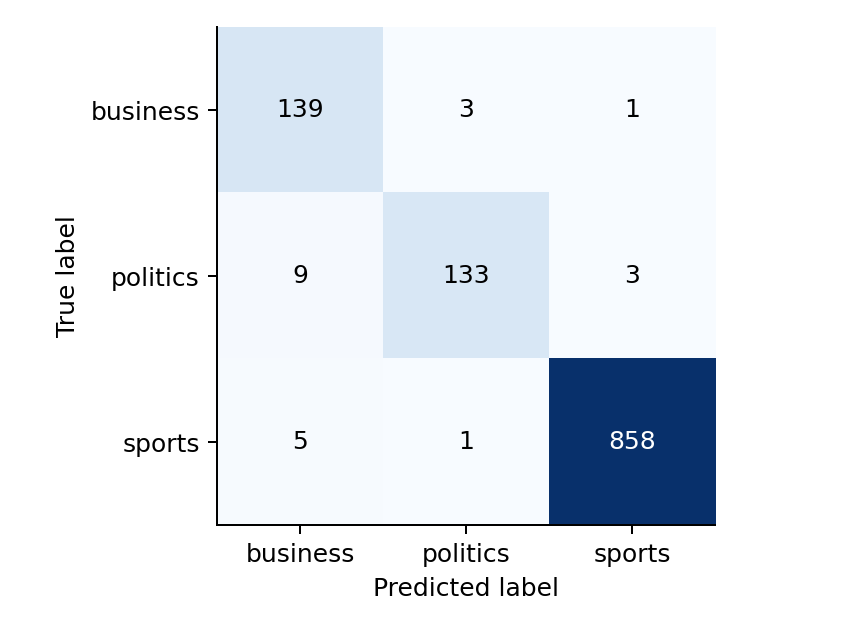
\includegraphics[width=0.74\linewidth]{bert_confusion.png}
\caption{BERT 测试集混淆矩阵}
\end{figure}

\begin{table}[H]
\centering\small
\setlength{\tabcolsep}{4pt}
\renewcommand{\arraystretch}{1.2}
\caption{BERT 测试集逐类指标}
\label{tab:result7}
\begin{tabularx}{\linewidth}{>{\hsize=1.03093\hsize\linewidth=\hsize\raggedright\arraybackslash}X>{\hsize=0.97938\hsize\linewidth=\hsize\raggedright\arraybackslash}X>{\hsize=0.97938\hsize\linewidth=\hsize\raggedright\arraybackslash}X>{\hsize=0.97938\hsize\linewidth=\hsize\raggedright\arraybackslash}X>{\hsize=1.03093\hsize\linewidth=\hsize\raggedright\arraybackslash}X}
\toprule
类别 & Precision & Recall & F1 & 样本数 \\
\midrule
business & 0.9085 & 0.9720 & 0.9392 & 143 \\
politics & 0.9708 & 0.9172 & 0.9433 & 145 \\
sports & 0.9954 & 0.9931 & 0.9942 & 864 \\
\bottomrule
\end{tabularx}
\end{table}

完全相同文本的交集数量：训练/验证 14，训练/测试 10，验证/测试 1（计不同文本数）。AG 与 NYT 的完全相同文本交集为 0。这些统计不涵盖改写或近重复新闻。

补充敏感性检查：排除与训练集文本完全相同的测试记录后，保留 1142 / 1152 条测试样本。以下仅重新计算已保存预测，不重新训练、不替代规定测试集主表。

\begin{table}[H]
\centering\small
\setlength{\tabcolsep}{4pt}
\renewcommand{\arraystretch}{1.2}
\caption{排除训练集重复文本后的补充指标}
\label{tab:result8}
\begin{tabularx}{\linewidth}{>{\hsize=1.08247\hsize\linewidth=\hsize\raggedright\arraybackslash}X>{\hsize=0.95876\hsize\linewidth=\hsize\raggedright\arraybackslash}X>{\hsize=0.95876\hsize\linewidth=\hsize\raggedright\arraybackslash}X}
\toprule
方法 & 排重后 Accuracy & 排重后 Macro-F1 \\
\midrule
Binary BoW & 0.9904 & 0.9750 \\
Frequency & 0.9886 & 0.9734 \\
TF-IDF & 0.9921 & 0.9809 \\
GloVe & 0.9877 & 0.9711 \\
Word2Vec AG & 0.9834 & 0.9573 \\
Word2Vec NYT & 0.9895 & 0.9727 \\
BERT & 0.9807 & 0.9582 \\
\bottomrule
\end{tabularx}
\end{table}


\section{复现与结论}

本次训练环境：Python 3.12.14；GPU 为 NVIDIA GeForce RTX 4060 Laptop GPU。所有结果使用同一保存划分，并通过逐条预测重算核验。

\begin{table}[H]
\centering\small
\setlength{\tabcolsep}{4pt}
\renewcommand{\arraystretch}{1.2}
\caption{实验运行环境}
\label{tab:result9}
\begin{tabularx}{\linewidth}{>{\hsize=1.01031\hsize\linewidth=\hsize\raggedright\arraybackslash}X>{\hsize=0.98969\hsize\linewidth=\hsize\raggedright\arraybackslash}X}
\toprule
依赖 & 实际版本 \\
\midrule
numpy & 2.2.6 \\
pandas & 2.2.3 \\
scikit-learn & 1.6.1 \\
gensim & 4.4.0 \\
torch & 2.6.0+cu124 \\
transformers & 4.51.3 \\
\bottomrule
\end{tabularx}
\end{table}

从仓库根目录执行以下命令（需安装 TeX Live 或 MiKTeX）：
\begin{lstlisting}[numbers=none,aboveskip=4pt,belowskip=4pt]
uv sync --frozen --python 3.12
uv run --frozen python scripts/run_all.py
\end{lstlisting}
分步说明见 \path{README.md}。报告使用 \path{report/} 中的南开大学模板，
通过 XeLaTeX 和 BibTeX 编译；LaTeX 正文、PDF 与 Markdown 来自同一实验结果。

可复核证据：results/split.json 保存划分与源文件 SHA-256；各方法 JSON 保存参数、验证和测试指标、混淆矩阵；*\_predictions.csv 保存原始行号、真实标签和预测标签；audit.json 保存独立指标核验及重复文本敏感性结果。预训练资源来源和 SHA-256 记录在 assets.json。

本次比较中，TF-IDF 达到最高测试 Macro-F1。结论仅适用于本数据、当前划分和给定超参数。未覆盖多随机种子、近重复去重和长文本 BERT 对照；这些是后续完善实验的方向，不作为本报告已经完成的实验。

\clearpage
\addcontentsline{toc}{section}{参考文献}
\bibliographystyle{plain}
\bibliography{references}
\end{document}
